	\section{Value Abstraction for DNN verification}

In this section, we describe different value (over-)abstractions on $\vz$ that are used by efficient algorithms to certify robustness around an input $\vx$. Over-abstractions of values include all values for $\vz$ in the neighbourhood of $\vx$, and thus a certificate for safety in the over-abstraction is a proof of safety for the original input $\vx$.

\subsection{The Box and DeepPoly Abstractions}



\begin{figure}[t!]
	\centering
	\begin{tikzpicture}
		
		\node[circle, draw= black, thick, minimum width = 20,
		minimum height = 20] (input1) {$n_1$};
		
		\node[circle, draw= purple, thick, minimum width = 20,
		minimum height = 20] (input2) at ($(input1) + (0,-1.5)$) {$n_2$};
		
		
		% Hidden layers
		
		\node (hidden10) at ($(input1) + (2.5,0.6)$) {$0$};
		
		\node (hidden20) at ($(input1) + (2.5,-1.5-0.6)$) {$0$};
		
		\node (hidden50) at ($(input1) + (7.5,0.6)$) {$0$};
		
		\node (hidden60) at ($(input1) + (7.5,-1.5-0.6)$) {$1.5$};
		
		
		\node[circle, draw= black, thick, minimum width = 20,
		minimum height = 20] (hidden1) at ($(input1) + (2.5,0)$) {$n_3$};
		\node[circle, draw= black, thick] (hidden2) at ($(input1) + (2.5,-1.5)$) {$n_4$};
		
		\node[circle, draw= black, thick, minimum width = 20,
		minimum height = 20] (hidden3) at ($(input1) + (5,0)$){$\hat{n}_3$};
		\node[circle, draw= black, thick] (hidden4) at ($(input1) + (5,-1.5)$) {$\hat{n}_4$};
		
		
		\node[circle, draw= blue, thick, minimum width = 20,
		minimum height = 20] (hidden5) at ($(input1) + (7.5,0)$){$n_5$};
		\node[circle, draw= black, thick] (hidden6) at ($(input1) + (7.5,-1.5)$) {$n_6$};
		
		
		
		
		% Output layer
		\node[circle, draw= black, thick, minimum width = 20,
		minimum height = 20] (output1) at ($(input1) + (10,0)$){$\hat{n}_5$};
		
		\node[circle, draw= black, thick, minimum width = 20,
		minimum height = 20] (output2) at ($(input1) + (10,-1.5)$){$\hat{n}_{6}$};
		
		
		% Connections
		
		\draw[->,thick] ($(input1) + (-1.5,0)$) -- (input1) node[midway, above] {$[-1,1]$};
		
		\draw[->,thick] ($(input1) + (-1.5,-1.5)$) -- (input2) node[midway, above] {$[-1,1]$};
		
		
		
		\draw[->,thick] (input1) -- (hidden1) node[near start, above] {$1$};
		\draw[->,thick] (input1) -- (hidden2)node[near start, above] {$1$};
		
		\draw[->,color=green, thick] (input2) -- (hidden1) node[near start, below] {$1$};
		\draw[->,color=red, thick] (input2) -- (hidden2)node[near start, below] {$-1$};
		
		
		
		
		
		\draw[->,color=green, thick] (hidden1) -- (hidden3) node[midway, above] {$\max(n_1,0)$};
		\draw[->,color=red, thick] (hidden2) -- (hidden4) node[midway, above] {$\max(n_2,0)$};
		
		
		
		
		
		\draw[->,color=green, thick] (hidden3) -- (hidden5) node[near start, above] {$1$};			
		\draw[->,thick] (hidden3) -- (hidden6) node[near start, above] {$0$};
		
		\draw[->,color=red, thick] (hidden4) -- (hidden5)node[near start, below] {$2$};
		\draw[->,thick] (hidden4) -- (hidden6)node[near start, below] {$1$};
		
		
		
		
		\draw[->,thick] (hidden5) -- (output1) node[midway, above] {$\max(n_5,0)$};
		\draw[->,thick] (hidden6) -- (output2) node[midway, above] {$\max(n_6,0)$};
		
		
	\end{tikzpicture}
	\caption{A DNN example from \cite{kpoly}: every neuron is separated into 2 nodes, $n$ pre- and $\hat{n}$ post-ReLU activation function. The pair $(n_2 n_3 n_5,n_2 n_4 n_5)$ in green and red is compensating (weights of paths are $1,-2$).}
	\label{fig1}
\end{figure}

The concept of value abstraction involves calculating upper and lower bounds for the values of certain neurons in a Deep Neural Network (DNN) when inputs fall within a specified range. This approach aims to assess the network's robustness without precisely computing the values for every input within that range.

Firstly, it's important to note that weighted sums represent a linear function, which can be explicitly expressed with relative ease. However, the ReLU (Rectified Linear Unit) function presents a challenge in terms of accurate representation. Although ReLU is a relatively straightforward piecewise linear function with two modes (one for $x<0$ and another for $x \geq 0$), it is not linear. The complexity arises when considering the compounded effects of the ReLU function across the various layers of a ReLU DNN. It's worth noting that representing $\ReLU(x)$ precisely is feasible when $x$ is "stable," meaning it's consistently positive or consistently negative, as there's only one linear mode involved in each scenario. Consequently, the primary challenge lies in addressing "unstable" neurons, where the linearity of the function does not hold consistently.


Consider the simpler abstraction, termed ``Box abstraction" \cite{deeppoly}: it inductively computes the bounds for each neuron in the subsequent layer independently. This is achieved by considering the weighted sum of the bounds from the previous layer, followed by clipping the lower bound at $\max(0,$ lower bound$)$ to represent the ReLU function, and so forth. For all $i$, define $x_i=\val_{\vx}(n_i)$, where $\vx=(x_1,x_2)$.

Taking the DNN example from Fig \ref{fig1}, assume $x_1,x_2 \in [-1,1]$. This implies that $x_3,x_4 \in [-2,2]$. After applying the ReLU function, $\hat{x}3,\hat{x}4$ are constrained to $[0,2]$, leading to $x_5 \in [0,6]$ and $x_6 \in [0,2]$. The bounds for $n_1, \ldots, n_4$ are exact, meaning for every $\alpha$ within the range, an input $\vy$ can be found such that $\val{\vy}(n_i)=\alpha$. However, this precision is lost from the next layer (beginning with $n_5, n_6$) due to potential dependencies among preceding neurons. For example, $n_3$ only attains the value $2$ when both $x_1$ and $x_2$ are $2$. In this case, $n_4$ would reach a value of $Val{(2,2)}(n_4)=0$. Consequently, it's implausible for $x_5=\Val_{\vx}(n_5)$ to reach $6$, as it would necessitate both $n_3$ and $n_4$ assuming the value $2$.

An extremely efficient algorithm that addresses some issues is "DeepPoly" \cite{deeppoly}, also independently discovered as the "CROWN" algorithm \cite{crown}. Instead of strict bounds, for each neuron $n$ in layer $k$, DeepPoly maintains two affine functions representing the lower and upper bounds of the neuron's value, based on inputs from the previous layer $k-1$. For instance, denote $f_i \leq x_i \leq g_i$ with, for example, $f_{3}(x_3)=f_4(x_4)=0$ and $g_3(x_3) = \frac{x_3+2}{2}$, $g_4(x_4) = \frac{x_4+2}{2}$. This leads to $x_5 \leq g_3(x_3) + 2 g_4(x_4) = \frac{x_3 + 2x_4 + 6}{2} = \frac{3x_1 - x_2 + 6}{2}\leq 5$.

For bounds $[\alpha,\beta]$ on $x_i$, the optimal linear function for the upper bound is $g_i(x_i)= \beta \frac{x_i-\alpha}{\beta-\alpha}$ for ReLU nodes. There are two options for the lower bound: $f^1_i(x_i) = 0$ or $f^2_i(x_i)=x_i$. DeepPoly selects between these based on the values of $\alpha$ and $\beta$ (for unstable neurons): if $|\alpha|\geq |\beta|$, then $f_i=f^1_i$ is chosen, otherwise, for $|\beta|>|\alpha|$, $f_i=f^2_i$ is selected. The variation, {\em $\overline{\mbox{DeepPoly}}$}, consistently chooses $f^1_i$, and never $f^2_i$. Contrary to DeepPoly, {\em $\overline{\mbox{DeepPoly}}$} encompasses the ``Box abstraction." For instance, with bounds $[-0.2,5]$ on $x_i$, it deduces $\ReLU(x_i) \in [0,5]$, whereas  DeepPoly without box abstraction algorithm would conclude $\ReLU(x_i) \in [-0.2,5]$.


\iffalse
\subsection{PRIMA and $\beta$-CROWN}
\fi

\subsection{MILP and LP encodings for DNNs}

At the other end of the spectrum, we find the Mixed Integer Linear Programming (MILP) value abstraction, which is a priori a complete method (albeit much slower than DeepPoly). 
Consider an unstable neuron $n \in[\alpha,\beta]$. The value $x$ of $\ReLU(n)$ can be encoded exactly in an MILP formula with one integer (actually even binary) variable $a$ valued in ${0,1}$, using 4 constraints \cite{MILP}:
\vspace{-0.1cm}
\begin{align*}
	\hat{x} \geq x \quad \wedge \quad \hat{x} \geq 0, \quad \wedge \quad \hat{x} \leq \beta \cdot a \quad \wedge \quad \hat{x} \leq x-\alpha \cdot (1-a)
\end{align*}

It can be shown that for all $x \in [\alpha,\beta] \setminus 0$, there exists a unique solution $(a,\hat{x})$ that meets these constraints, with $\hat{x}=\ReLU(x)$. Here, $a$ is 0 if $x < 0$, 1 if $x>0$, and can be either if $x=0$~\cite{MILP}. This encoding approach can be applied to every (unstable) ReLU node, and optimizing its value can help in certifying a given input. However, for networks with hundreds of nodes or more, the resulting MILP formulation will contain numerous integer variables and generally cannot be solved efficiently.

MILP instances can be linearly relaxed into LP over-abstraction, where variables originally restricted to integers in ${0,1}$ (binary) are relaxed to real numbers in the interval $[0,1]$, while maintaining the same encoding. As solving LP instances is polynomial time, this optimization is significantly more efficient. However, this efficiency comes at the cost of precision, often resulting in less stringent bounds. This approach is termed the {\em LP abstraction}

The following proposition shows that the LP abstraction refines the DeepPoly abstraction. 
The difference between the LP and the DeepPoly abstractions is that LP simultaneous considers the two linear lower bounding functions for the ReLU operation, namely $ReLU(x) \geq 0$ and $ReLU(x) \geq x$, while the DeepPoly abstraction restricts itself to the application of a single one of these linear bounding functions.
 

\begin{proposition}
	\label{LP}
	Given $x \in [\alpha,\beta]$ with $\alpha < 0 < \beta$, the following two systems of constraints 
	1) for LP and 2) for DeepPoly with both lower bounds are equivalent:
	\begin{align}
& \hat{x} \geq x \quad \wedge \quad \hat{x} \geq 0, \quad \wedge \quad \hat{x} \leq \beta \cdot a \quad \wedge \quad \hat{x} \leq x-\alpha \cdot (1-a), \, a \in [0,1]  \label{eq:lp}\\
&\hat{x} \geq x \quad \wedge \quad \hat{x} \geq 0 \quad \wedge \quad \hat{x} \leq \beta \frac{x-\alpha}{\beta-\alpha} \label{eq:deeppoly}
	\end{align} 
\end{proposition}

\begin{proof}
We need to show that the two upper bound constraints in Eq~\ref{eq:lp} is equivalent to the upper bound in Eq~\ref{eq:deeppoly}. To this end, we focus on the upper bound function in the linear variable $a \in  [0,1]$, with $x \in [\alpha,\beta]$ fixed. We have $\hat{x}$ in Eq~\ref{eq:lp} is upper bounded by $max_{a \in [0,1]} (min(\beta \cdot a, x - \alpha (1-a)))$, and this bound can be reached. Furthermore, 
	The function $\min(\beta \cdot a, x - \alpha (1-a))$ attains its maximum when $\beta \cdot a = x - \alpha (1-a)$, leading to the equation $(\beta - \alpha) a = x - \alpha$ and consequently $a = \frac{x - \alpha}{\beta-\alpha}$. This results in an upper bound of $\beta \cdot a = \beta \frac{x - \alpha}{\beta-\alpha}$ \qed
\end{proof}

\subsubsection*{Constraints for $\gamma$}

We could get the following constraints for $\gamma$, using $y_i$ and $\hat{y}_i$ to denote the $x_i-x_i'$ and $\hat{x}_i-\hat{x}_i'$:\begin{align*}
	\hat{y}_i \leq a \gamma_i \hspace*{2ex} &\wedge \hspace*{2ex}\hat{y} \geq y_i - a \gamma_i\\
	\hat{y}_i \geq (a-1) \gamma_i  \hspace*{2ex} &\wedge \hspace*{2ex} \hat{y} \leq y_i + (1-a) \gamma_i,
\end{align*} where $a$ is a binary variable, $\gamma_i$ is the upper bound of $x_i-x'_i$.


The following plot will show the above constraints:

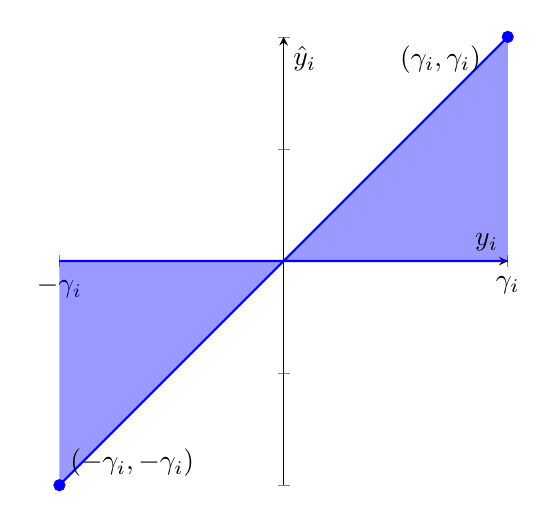
\begin{tikzpicture}
	\begin{axis}[
		xlabel={$y_i$},
		ylabel={$\hat{y}_i$},
		xmin=-2, xmax=2,
		ymin=-2, ymax=2,
		axis lines=center,
		samples=100, 
	 unit vector ratio=1 1 1, scale=1, xtick   = {-2,2},
	 xticklabels = {$-\gamma_i$,$\gamma_i$},
	 yticklabels = {},
		]
		\addplot[blue, thick, fill=blue, fill opacity=0.4] {x} \closedcycle; 
		\addplot[blue, thick] {0}; 
	
		\addplot[only marks, mark=*, mark size=2pt, blue] coordinates {(-2,-2)};
			\node[label={above:$(-\gamma_i,-\gamma_i)$}] at (axis cs: -1.35, -2.1) {};
			
				\addplot[only marks, mark=*, mark size=2pt, blue] coordinates {(2,2)};
			\node[label={above:$(\gamma_i,\gamma_i)$}] at (axis cs: 1.4, 1.5) {};
	\end{axis}
\end{tikzpicture}



The relation between $y_i$, $x'_i$ and $\hat{y}_i$ is $\hat{y}_i = \ReLU(x'_i+y_i)-\ReLU(x'_i).$ 


We can use the following extra constraints (besides 4 constraints about $\hat{x}_i'=\ReLU(x_i')$) to build this relation:


\begin{align*}
	&\hat{y}_i \geq -\hat{x}'_i \hspace*{1ex} \wedge \hspace*{1ex} \hat{y}_i \leq -\hat{x}'_i+a\beta_i  \hspace*{1ex}\wedge\hspace*{1ex} x_i'+y_i \leq a\beta_i \hspace*{1ex}\wedge\hspace*{1ex}  x_i'+y_i \geq (1-a)\alpha_i \\
	&\hat{y}_i \geq -\hat{x}'_i+(x_i'+y_i) \hspace*{1ex}\wedge\hspace*{1ex} \hat{y}_i \leq -\hat{x}'_i+(x_i'+y_i) +(a-1)\alpha_i \\
\end{align*} 


Moreover, we can add two more natural constraints: $x_i'+y_i \geq \alpha_i \hspace*{1ex}\wedge\hspace*{1ex}  x_i'+y_i \leq \beta_i.$



A more direct way to establish the constraints is as follows: \begin{align*}
	& y_i+x'_i \leq a\beta_i \quad\wedge \quad y_i+x'_i\geq (1-a)\alpha_i\\	
	& x_i' \leq a'\beta_i \quad\wedge \quad x_i'\geq (1-a')\alpha_i\\
	&\hat{y}_i \leq a\gamma_i \quad\wedge \quad	\hat{y}_i \geq -a'\gamma_i \\
	&	\hat{y}_i \leq y_i+(1-a)\gamma_i \quad\wedge \quad	\hat{y}_i \geq y_i - (1-a')\gamma_i \\
	&	\hat{y}_i \leq -x'_i+a\beta_i \quad\wedge \quad	\hat{y}_i \geq -x'_i+(1-a')\alpha_i \\
	&	\hat{y}_i \leq y_i+x'_i+(1-a)(-\alpha_i)\quad\wedge \quad	\hat{y}_i \geq y_i+x'_i+a'(-\beta_i) \\
\end{align*}The following two plots show its shape:

\hspace*{-10ex}
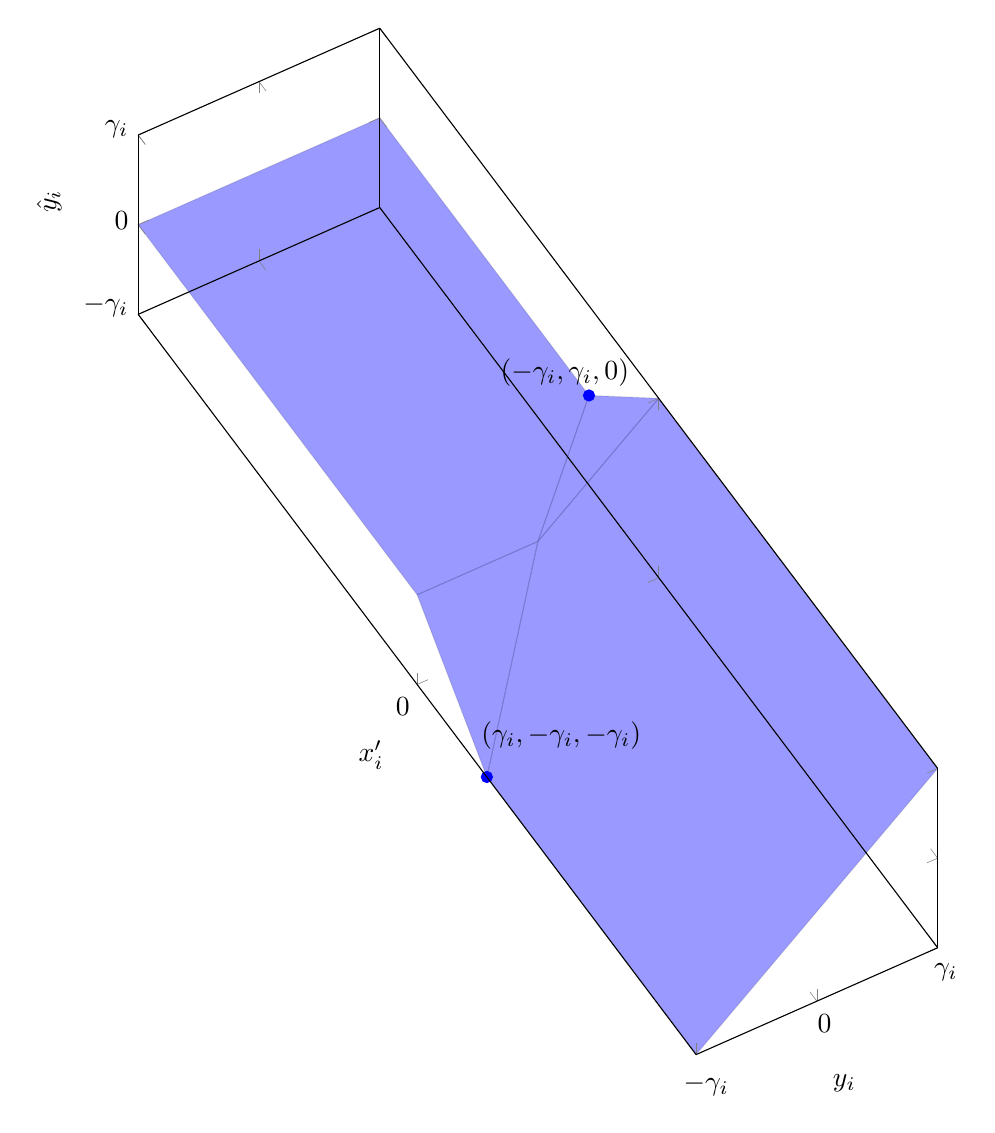
\begin{tikzpicture}
	\begin{axis}[	axis on top, xlabel = \(x'_i\),
		ylabel = {\(y_i\)}, zlabel = \(\hat{y}_i\),
				set layers=default,
	xmax = 4, xmin = -4,
ymax = 1, ymin = -1,		
zmax = 1, zmin = -1,
				unit vector ratio=1 1 1, scale=3,
				view={60}{50}, ytick   = {-1,0,1},
				yticklabels = {$-\gamma_i$,$0$,$\gamma_i$}, xtick = {0},
				xticklabels = {$0$}, ztick   = {-1,0,1},
				zticklabels = {$-\gamma_i$,$0$,$\gamma_i$},
				]
		\addplot3[fill=blue,opacity=0.1, fill opacity=0.4] 
		coordinates {
	 (0,0,0) (-1,1,0) (-4,1,0) (-4,-1,0) (0,-1,0) (0,0,0)
		};
		
		\addplot3[fill=blue,opacity=0.1, fill opacity=0.4	] 
		coordinates { (0,0,0) (0,1,1) (4, 1, 1) (4, -1, -1) (1,-1,-1) (0,0,0)
		};
		
		\addplot3[fill=blue,opacity=0.1, fill opacity=0.4	] 
		coordinates { (0,0,0)  (-1,1,0) (0,1,1) (0,0,0)
		};
		
			\addplot3[fill=blue,opacity=0.1, fill opacity=0.4	] 
		coordinates { (0,0,0)  (0,-1,0) (1,-1,-1) (0,0,0)
		};
		
		\addplot3[only marks, mark=*, mark size=2pt, blue] coordinates {(1,-1,-1)};
					\node[label={$(\gamma_i,-\gamma_i, -\gamma_i)$}] at (axis cs: 1.2, -0.5 ,-1) {};
					
			\addplot3[only marks, mark=*, mark size=2pt, blue] coordinates {(-1,1,0)};
		\node[label={$(-\gamma_i,\gamma_i, 0)$}] at (axis cs: -1, 0.8 ,0) {};			
		
	\end{axis}
\end{tikzpicture}



\hspace*{-15ex}
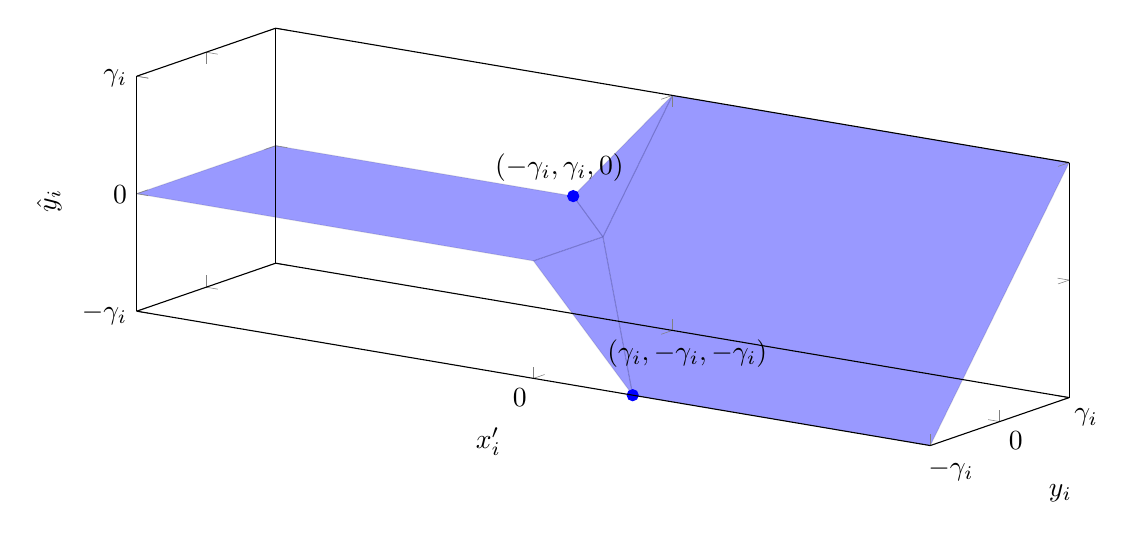
\begin{tikzpicture}
	\begin{axis}[	axis on top, xlabel = \(x'_i\),
		ylabel = {\(y_i\)}, zlabel = \(\hat{y}_i\),
		set layers=default,
				xmax = 4, xmin = -4,
		ymax = 1, ymin = -1,		
				zmax = 1, zmin = -1,
		unit vector ratio=1 1 1, scale=2.5,  ytick   = {-1,0,1},
		yticklabels = {$-\gamma_i$,$0$,$\gamma_i$}, xtick = {0},
		xticklabels = {$0$}, ztick   = {-1,0,1},
		zticklabels = {$-\gamma_i$,$0$,$\gamma_i$},
		view={35}{14},
		]
		\addplot3[ fill=blue,opacity=0.1, fill opacity=0.4] 
		coordinates {
			(0,0,0) (-1,1,0) (-4,1,0) (-4,-1,0) (0,-1,0) (0,0,0)
		};
		
		\addplot3[	fill=blue,opacity=0.1, fill opacity=0.4] 
		coordinates { (0,0,0) (0,1,1) (4, 1, 1) (4, -1, -1) (1,-1,-1) (0,0,0)
		};
		
		\addplot3[	fill=blue,opacity=0.1, fill opacity=0.4	] 
		coordinates { (0,0,0)  (-1,1,0) (0,1,1) (0,0,0)
		};
		
		\addplot3[	fill=blue,opacity=0.1, fill opacity=0.4	] 
		coordinates { (0,0,0)  (0,-1,0) (1,-1,-1) (0,0,0)
		};
		
			\addplot3[only marks, mark=*, mark size=2pt, blue] coordinates {(1,-1,-1)};
		\node[label={$(\gamma_i,-\gamma_i, -\gamma_i)$}] at (axis cs: 1.2, -0.5 ,-1) {};
		
		\addplot3[only marks, mark=*, mark size=2pt, blue] coordinates {(-1,1,0)};
		\node[label={$(-\gamma_i,\gamma_i, 0)$}] at (axis cs: -1, 0.8 ,0) {};			
		
	\end{axis}
\end{tikzpicture}


%\begin{tikzpicture}[
%	declare function={
%		f(\x,\y)=max((\x+\y),0)-max(\x,0);
%	}]
%	\begin{axis}[axis lines=center,
%		axis on top,
%		set layers=default,
%		xrange=-3:3,
%		yrange=-2:2,
%		unit vector ratio=1 1 1,% <- HERE (taken from Phelype Oleinik's deleted answer)
%		scale=3 %<- added to compensate for the downscaling
%		% resulting from unit vector ratio=1 1 1
%		]
%		\addplot3[
%		domain=-3:3,
%		domain y=-1:1, surf,
%		samples=40,
%		samples y=40,
%		] {f(\x,\y)};
%	\end{axis}
%\end{tikzpicture}
